\textbf{Результаты работы.}
\begin{enumerate}
	\item \textit{Представить разностный аналог краевого условия при $x = l$
	и его краткий вывод интегро-интерполяционным методом.}
	
	Проинтегрируем исходное выражение на отрезке $[x_{N-1/2}; x_{N}]$.
	\begin{equation*}
		\int_{x_{N-1/2}}^{x_{N}} \frac{dF}{dx}dx + \int_{x_{N-1/2}}^{x_{N}} f(T(x))dx = 0
	\end{equation*}
	
	Вычислим интегралы:
	\begin{equation*}
		-(F_{N} - F_{N-1/2}) + \frac{h}{4}(f(t_{N}) + f(t_{N-1/2})) = 0
	\end{equation*}
	
	Подставляя $F_N$ и $F_{N-1/2}$ заданные правым краевым условием:
	\begin{equation*}
		-\alpha(t_N - T0) + \chi_{N-1/2} \dfrac{t_{N-1} - t_{N}}{h}
		+ \frac{h}{4}(f(t_{N}) + f(t_{N-1/2})) = 0
	\end{equation*}
	
	Получаем $K_N t_{N-1} + M_N t_{N} = P_N$, где 
	\begin{equation*}
		\begin{cases}
			K_N = \frac{\chi_{N-1/2}}{h} \\ 
			M_N = -\alpha - \frac{\chi_{N-1/2}}{h}\\
			P_N = -\alpha \cdot T0 - \frac{h}{4}(f(t_{N}) + f(t_{N-1/2}))\\
		\end{cases}
	\end{equation*}

	Для удобства умножим все коэффициенты на $-h$. В полученном выражении, учитывая, что $h \rightarrow 0$ принебрегаем членами с $h^2$.
	
	\begin{equation*}
		\begin{cases}
			K_N = - \chi_{N-1/2} \\ 
			M_N = \alpha \cdot h + \chi_{N-1/2}\\
			P_N = \alpha \cdot T0 \cdot h\\
		\end{cases}
	\end{equation*}
	
	\newpage
	\item \textit{График зависимости температуры T(x) от координаты x при заданных выше параметрах.\\
	Выяснить, как сильно зависят результаты расчета T(x) и необходимое для этого количество итераций от начального распределения температуры и шага сетки.}
	
	\begin{figure}[h]
		\begin{center}
			{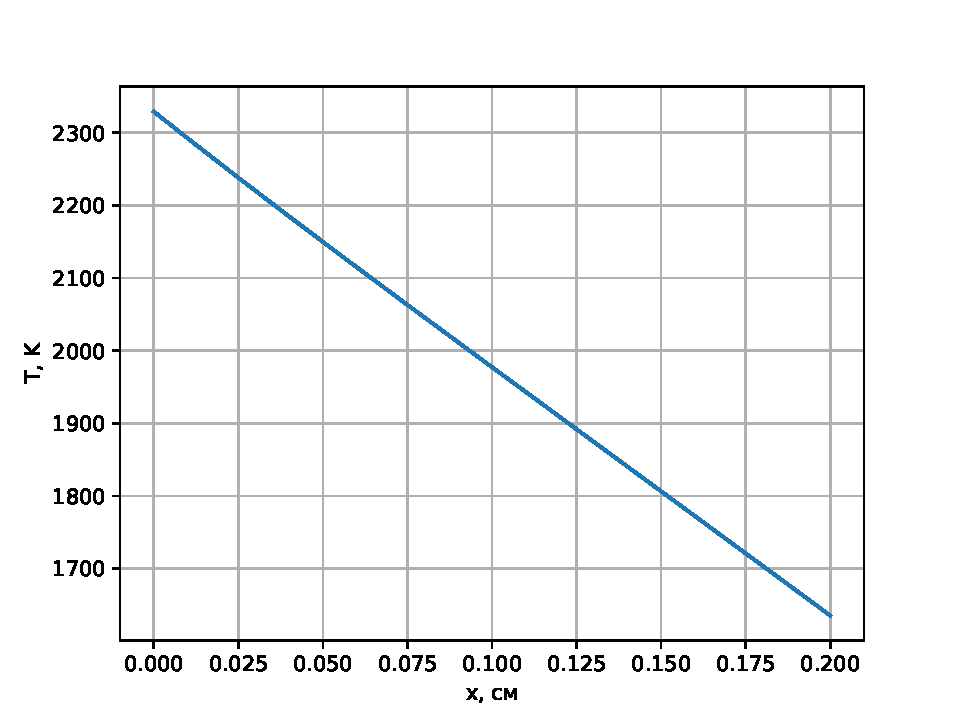
\includegraphics[height=9.5cm, width = 18cm]{../pictures/Figure_1}}
			\caption{Задание 2}
		\end{center}
	\end{figure}

	\qquadПри увеличении на порядок шага, использованного в работе, ухудшаются результаты работы программы: меняются значения температур левого/правого края. Уменьшение шага незначительно влияет на результат. Количество итераций практически не меняется. Начальное распределение температуры не влияет на результат. Разница в количестве итераций между достаточно приближенным распределением (от 2400 до 1600) и удаленным распределением (от 300 до 300) равна примерно в 3-4 итерации.
	
	\newpage
	\item \textit{График зависимости T(x) при $F_0 = -10$ Вт/см2.} 
	
	\begin{figure}[h]
		\begin{center}
			{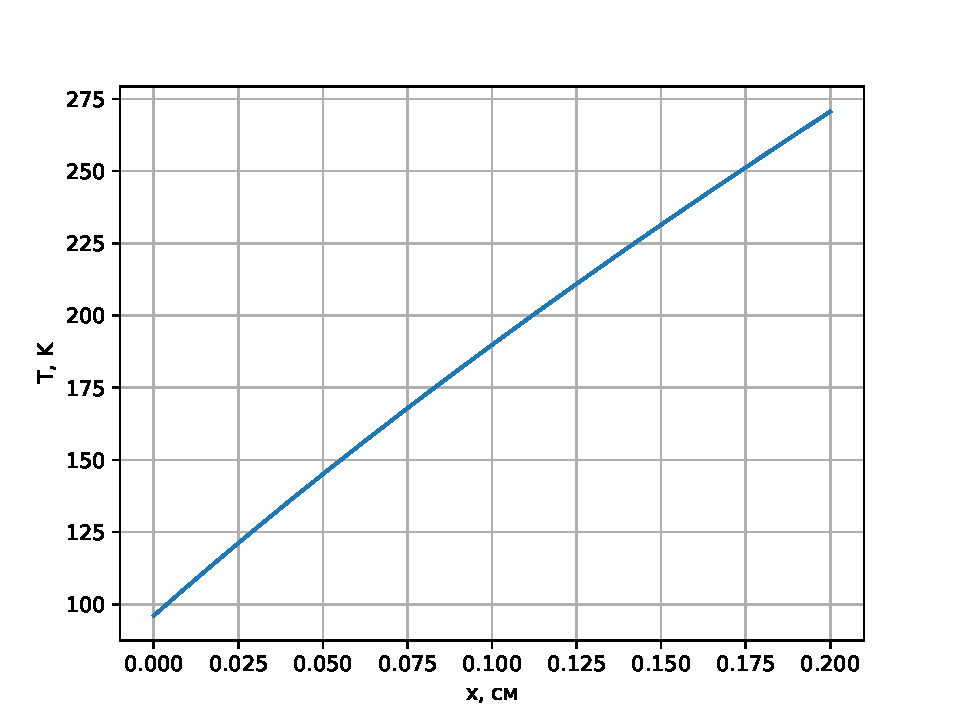
\includegraphics[height=9.5cm, width = 18cm]{../pictures/Figure_2}}
			\caption{Задание 3}
		\end{center}
	\end{figure}
	
	\newpage
	\item \textit{График зависимости T(x) при увеличенных значениях $\alpha$ (например, в 3 раза). Сравнить с п.2.}
	
	\begin{figure}[h]
		\begin{center}
			{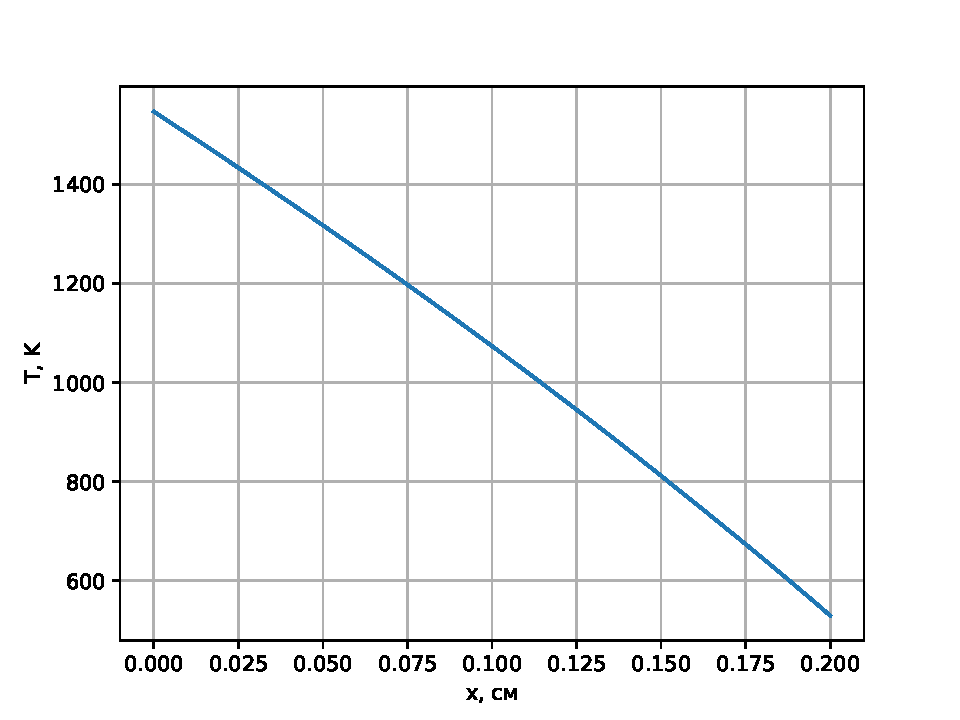
\includegraphics[height=9.5cm, width = 18cm]{../pictures/Figure_3}}
			\caption{Задание 4}
		\end{center}
	\end{figure}

	\qquadПри $\alpha$, увеличенном в 3 раза, можно заметить, что снизился общий уровень температуры графика, температура правой границы приблизилась к T0. Это обусловено физической природой модели: увеличился теплосъём на правой границе.\\
	
	\newpage
	\item \textit{График зависимости T(x) при $F_0 = 0$.}
	
	\begin{figure}[h]
		\begin{center}
			{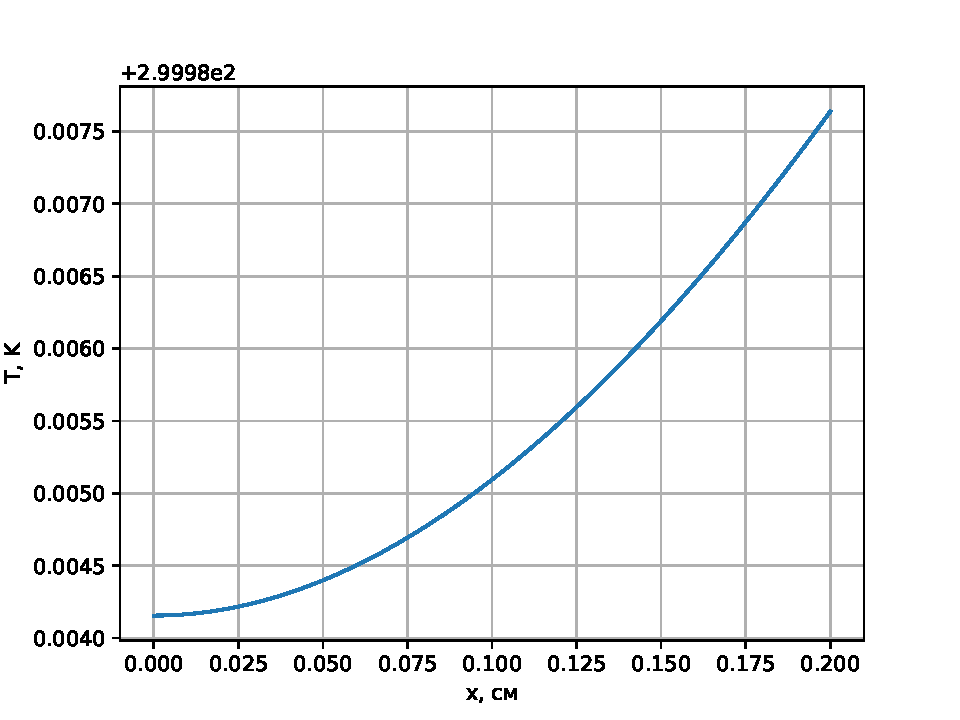
\includegraphics[height=9.5cm, width = 18cm]{../pictures/Figure_4}}
			\caption{Задание 5}
		\end{center}
	\end{figure}
	
	\item \textit{Для указанного в задании исходного набора параметров привести данные по балансу энергии, т.е. значения величин
	\begin{equation}\label{formula7}
		f_1 = F_0 - \alpha(T(l) - T_0)
	\end{equation}
	и
	\begin{equation}\label{formula8}
		f_2 = 4n_p^2 \sigma \int_0^l k(T(x))(T^4(x) - T_0^4)dx
	\end{equation}
	Каковы использованные в работе значения точности выхода из итераций
	$\varepsilon_1$ (по температуре) и
	$\varepsilon_2$ (по балансу энергии)?}
	
	\begin{table}[h]\label{table_2}
		\caption{Задание 6}
		\centering
		\begin{tabular}{|c|c|c|}
			\hline
			Номер итерации & $f_1$ & $f_2$\\
			\hline
			$0$ &$22.0000$ &$23.1089$ \\
			\hline
			$1$ &$21.9726$ &$22.5581$ \\
			\hline
			$2$ &$21.9020$ &$22.1540$ \\
			\hline
			$3$ &$21.8067$ &$21.8528$ \\
			\hline
			$4$ &$21.6985$ &$21.6249$ \\
			\hline
			$5$ &$21.5856$ &$21.4501$ \\
			\hline
			$6$ &$21.4729$ &$21.3143$ \\
			\hline
			$7$ &$21.3639$ &$21.2074$ \\
			\hline
			$8$ &$21.2604$ &$21.1222$ \\
			\hline
			$9$ &$21.1635$ &$21.0534$ \\
			\hline
			$10$ &$21.0738$ &$20.9974$ \\
			\hline
			$11$ &$20.9914$ &$20.9511$ \\
			\hline
			$12$ &$20.9162$ &$20.9125$ \\
			\hline
		\end{tabular}
	\end{table}

	$\varepsilon_1$ = 2.5e-4 \\
	$\varepsilon_2$ = 2.5e-4
	

\end{enumerate}